\section{Der Abtastsatz}

\begin{definition}\leavevmode
\begin{enumerate}
\item Eine Funktion $ f \in L_{1}(\R) $ heißt \emph{bandbeschränkt} mit \emph{Bandbreite $ t $} oder
  kurz \emph{$ T $-bandbeschränkt}, wenn
  \[
    \widehat{f}(\xi) = 0, \qquad \xi \notin [-T,T].
  \]
  Oder anders formuliert: Eine Funktion $ f \in L_{1}(\R) $ ist bandbeschränkt, wenn $ \widehat{f} $
  endlichen Träger besitzt.
\item Der \emph{Sinus Cardinalis} oder $ \sinc $-Funktion ist definiert als
  \[
    \sinc(x) \coloneqq \begin{cases}
      \frac{\sin(\pi x)}{\pi x}, & x \in \R \setminus \{ 0 \}, \\
      1, & x = 0.
    \end{cases}
  \]
\end{enumerate}
\end{definition}

\begin{remark}[Bandbeschränktheit]
Ist eine Funktion $ T $-bandbeschränkt, dann ist sie auch gleichzeitig $ T + n $-bandbeschränkt für
jedes $ n > 0 $. D.h.\ es gibt eigentlich gar nicht \emph{die} Bandbreite einer Funktion.
\end{remark}

\begin{remark}[Sinus Cardinalis]\leavevmode
\begin{itemize}
\item Der Name stammt daher, dass die Funktion an allen ganzzahligen Stellen entweder den Wert 
  $ 0 $ oder $ 1 $ annimmt. Abbildung~\ref{fig:sinc} zeigt den Verlauf der $ \sinc $-Funktion.
  \begin{figure}[ht]
  \centering
  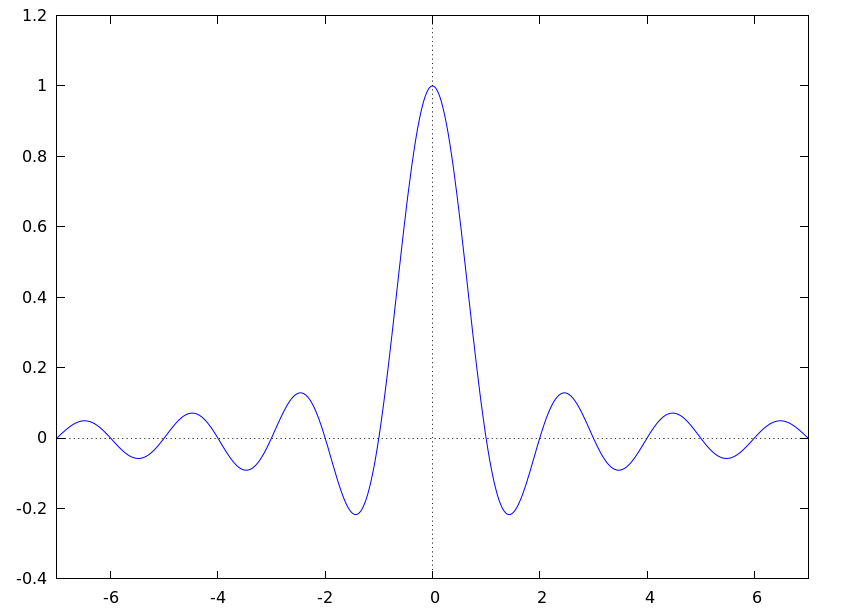
\includegraphics[width=0.7\textwidth]{Bilder/sinc}
  \caption{Plot der $ \sinc $-Funktion auf dem Intervall $ [-7,7] $.}
  \label{fig:sinc}
  \end{figure}
\item Fun fact: Es gilt
  \[
    \int_{\R} \sinc(x) \dif x = 1 \quad \text{und damit} \quad
    \int_{\R} \sinc(x / \pi) \dif x = \pi.
  \]
\item Die $ \sinc $-Funktion ist i.W.\ bis auf Normierung die Fourier-Transformierte der
  Rechtecksfunktion. Damit ist der $ \sinc $ der ideale Tiefpassfilter (aus Sicht des
  Frequenzbereichs).
\item Es kann aber gezeigt werden, dass $ \sinc \notin L_{1}(\R) $, weswegen der ideale 
  Tiefpassfilter nur näherungsweise implementiert werden kann. Es gilt aber
  $ \sinc \in L_{2}(\R) $, was u.a.\ ein Grund dafür ist, die Fourier-Transformation auf dem
  $ L_{2}(\R) $ einzuführen. Für Beweis siehe Anhang~\ref{sec:sincproofs}.
\end{itemize}
\end{remark}

\begin{proposition}[Abtastsatz von Shannon]
Ist $ f \in L_{1}(\R) $ eine $ T $-bandbeschränkte Funktion und ist $ h < h^{*} = \pi / T $, dann 
ist
\[
  f(x) = \left( (S_{h} \ f) * \sinc \right) \left( \frac{x}{h} \right) 
       = \sum_{k \in \Z} f(hk) 
           \frac{\sin \left( \pi \left( \frac{x}{h} - k \right) \right)}
                {\pi \left( \frac{x}{h} - k \right)}.
\]
\end{proposition}

\begin{remark}[Abtastsatz von Shannon]
Ein paar Anmerkungen dazu:
\begin{itemize}
\item Der Abtastsatz liefert uns eine Formel, wie man das ursprüngliche Signal $ f $ aus einer
  Abtastung $ S_{h} \ f $ mithilfe der $ \sinc $-Funktion\footnote{Der $ \sinc $ ist schließlich 
  der ideale Interpolationskern für ganzzahlige Stützstellen. Sagt zumindest Wikipedia.} 
  rekonstruieren kann. Allerdings besitzt der $ \sinc $ unendlichen Träger und fällt nur linear ab, 
  sodass man in der Praxis wohl lieber mit anderen Funktionen arbeiten sollte. 
\item Voraussetzung dafür, dass die Rekonstruktion wie gewünscht funktioniert, ist, dass\dots
  \begin{itemize}
  \item $ f $ nicht zu große Frequenzen enthalten darf (das ist die Forderung der
    $ T $-Bandbeschränktheit). Sonst könnte es potentiell unendlich hohe Frequenzen geben und dann
    müsste die Schrittweite für die Abtastung unendlich nahe bei der $ 0 $ liegen, was nicht
    wirklich Sinn macht.
  \item die Schrittweite $ h $ an den Parameter $ T $ angepasst wird, um eine ausreichend große 
    Zahl an Abtastpunkten zu erreichen. Sonst hat man zu wenig Information, um $ f $ eindeutig 
    rekonstruieren zu können (siehe Abbildung~\ref{fig:aliasing}). Die unerwünschten Effekte, die 
    aus einer Unterabtastung resultieren, bezeichnet man als \emph{Aliasing}. Bei Bildern können 
    dadurch z.B.\ neue Strukturen auftreten, die im Original gar nicht enthalten sind.
  \end{itemize}
  Die Kopplung von Bandbreite und Abtastfrequenz ist also wirklich essentiell. 
\item Die Abtastfrequenz $ 1 / h $ wird auch als \emph{Nyquist-Frequenz} bezeichnet.
\item Wählt man die Abtastfrequenz $ k $-mal so hoch wie nötig, so spricht man auch von
  $ k $-fachem Oversampling.
\item \TODO{Skript S.33f. und Bild auf Seite 34}
\end{itemize}
\end{remark}

\begin{figure}[ht]
	\centering
  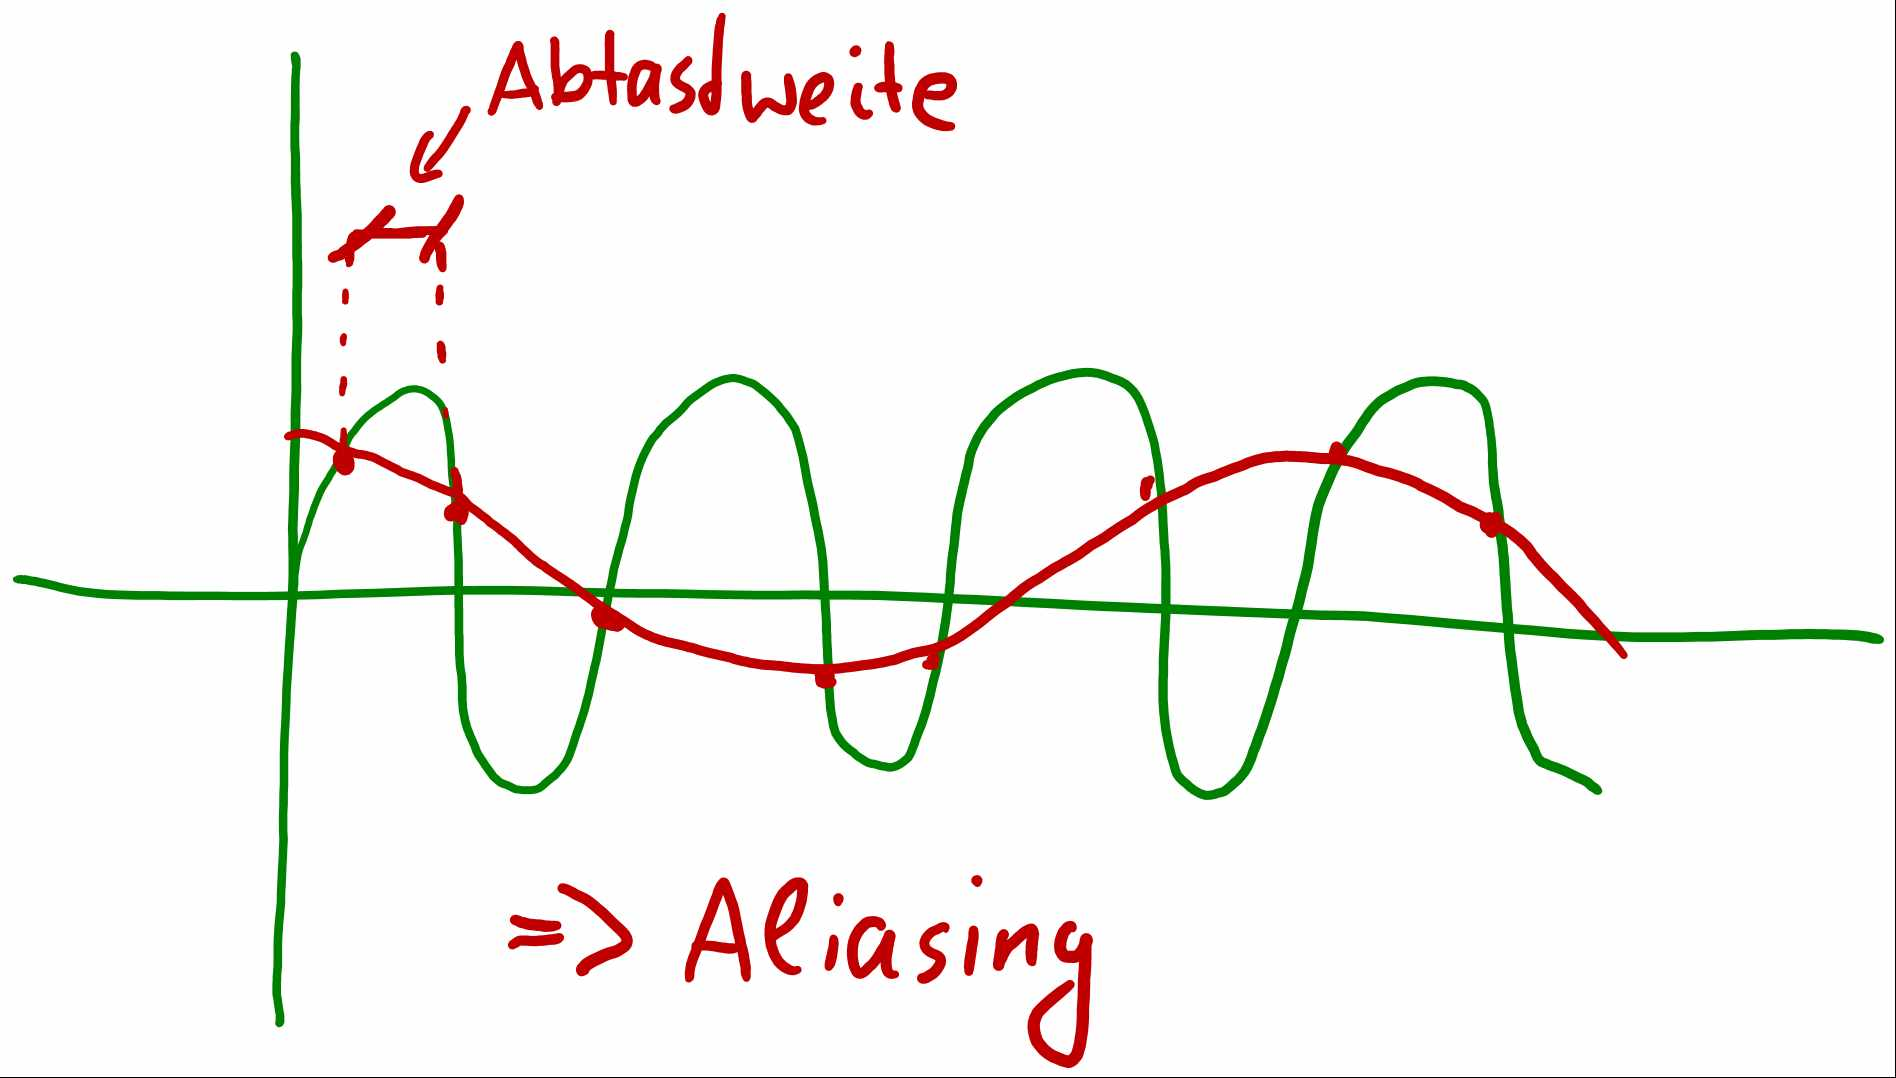
\includegraphics[width=0.7\textwidth]{Bilder/Aliasing}
	\caption{Aus der gegebenen Menge an äquidistanten Abtastpunkten kann die hochfrequente 
	grüne Funktion nicht rekonstruiert werden, da auch eine zweite Funktion (rot) gefunden werden 
	kann, welche den Punkten genau entspricht. Die Abtastweite wurde zu groß gewählt.}
	\label{fig:aliasing}
\end{figure}